\begin{song}{title=\centering 1. signální \\\normalsize Chinaski  \vspace*{-0.3cm}}  %% sem se napíše jméno songu a autor
\moveright \stred \vbox{      %Varianta č. 1  ---> Jeden sloupec zarovnaný na střed	

\sloka 
	^{Emi}Až si ^{G{\color{white}\_\_}}zejtra ráno ^{C}řeknu zase 

	^{Emi}jednou provždy dost,

	^{G{\color{white}\_\_\_}}právem se mi ^{C{\color{white}\_\_}}budeš tiše ^{Emi}smát

	jak omluvit si svoji slabost,

	nenávist a zlost,

	když za všechno si můžu vlastně sám. 

\refren
	^{Ami}Za spoustu dní možná za ^{C{\color{white}\_\_\_}}spoustu let 

	až se mi ^{G{\color{white}\_\_\_}}rozední, budu ti ^{D{\color{white}\_\_\_}}vyprávět 

	na 1. ^{Ami{\color{white}\_}}signální, jak jsem ^{C{\color{white}\_\_\_}}vobletěl svět, 

	jak tě to ^{G{\color{white}\_\_\_}}vomámí a ^{D{\color{white}\_\_\_}}nepustí zpět.

	Jaký si to ^{F{\color{white}\_\_}}uděláš, ^{B{\color{white}\_\_}}takový to ^{Dmi}máš. 

	Jaký si to ^{F{\color{white}\_\_}}uděláš, ^{B{\color{white}\_\_}}takový to ^{Dmi}máš. 

\sloka
	Až se dneska večer budu tvářit
	
	zas jak Karel Gott, 
	
	budu zpívat vampamtydapam,
	
	všechna sláva polní tráva,
	
	ale peníz přijde vhod,
	
	jak jsem si to uďál tak to mám.

\refren

\sloka Nana\dots

}
\setcounter{Slokočet}{0}
\end{song}


\begin{figure}[h]
\centering
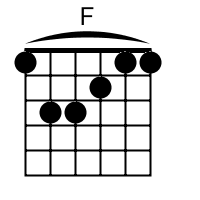
\includegraphics[scale=1.5]{../Akordy/f.png}
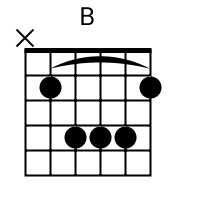
\includegraphics[scale=1.5]{../Akordy/h.png}
\end{figure}
